\documentclass[a4paper,12pt]{article}

% Encoding & fonts 
\usepackage[utf8]{inputenc}
\usepackage[T1]{fontenc}

% Page layout 
\usepackage[a4paper,left=2cm,right=2cm,top=2cm,bottom=2cm,bindingoffset=0cm]{geometry}

% Graphics & figures
\usepackage{graphicx}
\graphicspath{{../figures/}}
\usepackage{float}
\usepackage{subcaption}

% Mathematics 
\usepackage{amsmath}
\usepackage{amssymb}
\usepackage{bm}    

% Tables 
\usepackage{tabularx}
\usepackage{booktabs}
\usepackage{multirow}
\usepackage{makecell}

% Colors 
\usepackage{xcolor}
\usepackage{xkcdcolors}

% Code listings
\usepackage{listings}
\lstset{
    breaklines=true,
    breakatwhitespace=true,
    basicstyle=\ttfamily\small,
    frame=single
}

% Algorithms 
\usepackage{algorithm}
\usepackage{algpseudocode}

% Miscellaneous
\usepackage{cancel}
\usepackage{comment}
\usepackage{enumitem}
\usepackage{todonotes}
\usepackage{pdfpages}
\usepackage{lipsum}     
\usepackage{siunitx}    
\usepackage{csquotes}   
\usepackage{microtype}

\usepackage[
    colorlinks  = true,
    pdfstartview= FitV,
    linkcolor   = xkcdBlue,
    citecolor   = xkcdRed,
    urlcolor    = xkcdGreen
]{hyperref}

\usepackage[backend=biber, style=ieee]{biblatex}
\addbibresource{ref.bib}

\usepackage{fancyhdr}
\fancypagestyle{firstpage}{
    \fancyhf{}
    \setlength{\headheight}{14pt}
    \setlength{\headsep}{0.2in}
    \lhead{\small AE4889 -- \textit{MIMOSA}}
    \rhead{\small Daniel Pérez Trias}                       
    \cfoot{\thepage}
}
\pagestyle{firstpage}  

\usepackage{titlesec}
\titlespacing*{\section}{0pt}{1pt}{1pt}
\titlespacing*{\subsection}{0pt}{1pt}{1pt}

\setlength{\textfloatsep}{2pt}
\setlength{\intextsep}{2pt}
\setlength{\floatsep}{2pt}

\usepackage{glossaries}
\makeglossaries

\newacronym{mimosa}{MIMOSA}{MIssion to Mars with a sOlar SAil}
\newacronym{jpl}{JPL}{Jet Propulsion Laboratory}
\newacronym{cr3bp}{CR3BP}{Circular Restricted Three-Body Problem}
\newacronym{aep}{AEP}{Artificial Equilibrium Point}
\newacronym{mpo}{MPO}{Mars Parking Orbit}

\begin{document}

\thispagestyle{empty}
\vspace*{2cm}
\begin{center}
    {\LARGE \textbf{AE4889 \\ Special Topics in Astrodynamics} \\ \textit{MIMOSA} -- MIssion to Mars with a sOlar SAil \par}
    \vspace{1cm}
    {\Large Daniel Pérez Trias -- 6565158 \par}
    {\Large Delft, \today\par}
    \vspace{1em}
    {\large \href{https://github.com/dptrias/SpecialTopicsAstrodynamics}{\texttt{github.com/dptrias/SpecialTopicsAstrodynamics}} \par}
    \vspace{1em}
    {\normalsize \textit{Collaborated with:} \par}
    \vspace{0.5em}
    {\normalsize
        \begin{minipage}{0.4\textwidth}
            \begin{itemize}[label=\textendash,leftmargin=*]
                \item Andreu Craus Vidal
                \item Rodrigo Duarte Soares
                \item Ismael Gallo López
            \end{itemize}
        \end{minipage}
    \par}
    \vspace{4em}
    \begin{tabular}{ll}
        Personal problem specification & \\
        \toprule
        \textbf{Parameter} & \textbf{Value} \\
        \midrule
        Sun--Earth Lagrange point     & L$_2$ \\
        Sun--Mars Lagrange point    & L$_2$ \\
        Shift in Lagrange points     & $0.0005$ \\
        Radius Martian parking orbit & $\SI{306 666}{\km}$ \\
        Lightness number             & $0.025$ \\
        \bottomrule
    \end{tabular}
\end{center}


\newpage

% --- Table of contents -------------------------------------------------------
\thispagestyle{empty}
\tableofcontents
\newpage

% --- List of acronyms --------------------------------------------------------
\printglossary[type=\acronymtype, title=List of Acronyms]
\addcontentsline{toc}{section}{List of Acronyms}
\newpage

% --- List of figures ---------------------------------------------------------
% \listoffigures
% \addcontentsline{toc}{section}{List of Figures}
% \newpage
% 
% % --- List of tables ----------------------------------------------------------
% \listoftables
% \addcontentsline{toc}{section}{List of Tables}
% \newpage
% 

% --- Start main body with page counter reset ---------------------------------
\setcounter{page}{1}

% INTRODUCTION
\phantomsection
\section*{WP1 Sun--Earth and Sun--Mars Lagrange points}
\addcontentsline{toc}{section}{WP1 Sun--Earth and Sun--Mars Lagrange points}
\label{sec:wp1}

\begin{enumerate}
    \item[\textbf{1.1a}] The Lagrange points of the Sun--Earth and Sun--Mars systems are computed using Newton's method over equation \eqref{eq:colinear_lagrange}, which is derived from the \acrfull{cr3bp}. The resulting dimensionless coordinates of the colinear Lagrange points (L$_2$) are presented in Table \ref{tab:lagrange_points}.
    \begin{equation}
        \label{eq:colinear_lagrange}
        x - \frac{1-\mu}{(x+\mu)^2} - \frac{\mu}{(x-1+\mu)^2} = 0
    \end{equation}
    \vspace{1em}
    \begin{table}[htbp]
        \centering
        \caption{Dimensionless coordinates $(x_i, y_i, z_i)$ of the Sun--Earth and Sun--Mars
        colinear Lagrange points in their respective synodic reference frames, obtained
        from the solution of the circular restricted three-body problem using a Newton method.}
        \label{tab:lagrange_points}
        \begin{tabular}{lccc}
            \toprule
            \textbf{Lagrange point} & $x_i$ [LU] & $y_i$ [LU] & $z_i$ [LU]\\
            \midrule
            Sun--Earth L$_2$ & 1.01009044 & 0 & 0 \\
            Sun--Mars L$_2$  & 1.00476311 & 0 & 0 \\
            \bottomrule
        \end{tabular}
    \end{table}
    
    \item[\textbf{1.1b}] For verification purposes, the dimensionless coordinates of the colinear Lagrange points are 
    also extracted from the \href{https://ssd.jpl.nasa.gov/tools/periodic_orbits.html\#/periodic}{\acrfull{jpl} Solar System 
    Dynamics three-body periodic orbits tool}, which are presented in Table \ref{tab:lagrange_points_jpl}.
    It can be observed that for the represented number of digits, the values are identical, with differences on the 
    order of $10^{-9}$ LU, likely due to shared system parameters. \textit{(50 words)}
    \vspace{1em}
    \begin{table}[htbp]
        \centering
        \caption{Dimensionless $x$ coordinates of the Sun--Earth and Sun--Mars
        colinear Lagrange points in their respective synodic reference frames per JPL and their absolute differences w.r.t. the values obtained from the Newton method.}
        \label{tab:lagrange_points_jpl}
        \begin{tabular}{lcc}
            \toprule
            \textbf{Lagrange point} & $x_i$ [LU]& $\Delta x_i$ [LU] \\
            \midrule
            Sun--Earth L$_2$ & $1.01009044$ & $4.21585256 \times 10^{-9}$ \\
            Sun--Mars L$_2$  & $1.00476311$ & $3.32491457 \times 10^{-9}$ \\
            \bottomrule
        \end{tabular}
    \end{table}

    \item[\textbf{1.2}] A greater value of $\mu$ means the primary's gravitational pull weakens ($1-\mu$) while the secondary's strengthens($\mu$).
    Since L$_2$ sits close to the secondary, this increase is more strongly felt there and must be offset by moving the point further from it. 
    Increasing this distance has two compensating effects: it reduces the secondary's pull more sharply than the primary's (due to proximity), 
    and it increases the centrifugal acceleration, which opposes both gravitational contributions. The net result is that a more massive secondary, 
    as in the Sun--Earth system, pushes L$_2$ further from the planet than in the Sun--Mars case. \textit{(99 words)}

\end{enumerate}

\newpage
\phantomsection
\section*{WP2 Artificial Lagrange points}
\addcontentsline{toc}{section}{WP2 Artificial Lagrange points}
\label{sec:wp2}
\begin{enumerate}
    \item[\textbf{2.1a}] See Table \ref{tab:lightness_number}. 
    \vspace{1em}
    \begin{table}[htbp]
        \centering
        \caption{Required lightness number to achieve the specified shift in the Lagrange points.}
        \label{tab:lightness_number}
        \begin{tabular}{lp{5cm}c}
            \toprule
            \textbf{Lagrange point} & \textbf{Shift in Lagrange point along the Sun-Planet line} & \textbf{Required lightness number,} $\beta$ \\
            \midrule
            Sun--Earth L$_2$ & $0.0005$ & $4.76757628 \times 10^{-3}$ \\
            Sun--Mars L$_2$  & $0.0005$ & $5.06104189 \times 10^{-3}$ \\
            \bottomrule
        \end{tabular}
    \end{table} \par

    With respect to feasibility, NASA's \textit{ACS3} (currently in orbit), based on DCB deployable composite boom technology, 
    has a lightness number $\beta = 0.025$ \cite{wilkie2021ACS3}, an order of magnitude above the required values. This confirms that 
    the artificial Lagrange point shifts studied are achievable with current solar sail technology. \textit{(47 words)}

    \item[\textbf{2.1b}] Since the required shift is along the Sun--planet line, and all forces at the collinear Lagrange points are 
    aligned along this axis, the sail orientation needed to achieve the desired shift is likewise along this line. As the spacecraft 
    moves sunward from L$_2$, the gravitational pulls of both bodies strengthen while the centrifugal acceleration diminishes, requiring 
    a compensating force directed away from the Sun. This uniquely determines the sail orientation, with the sail normal away from the Sun. \textit{(80 words)}
    \vspace{1em}
    \begin{table}[htbp]
        \centering
        \caption{Required sail orientation to achieve the required shift in the Lagrange points.}
        \label{tab:sail_orientation}
        \begin{tabular}{lccc}
            \toprule
            \textbf{Lagrange point} & $n_{x,i}$ & $n_{y,i}$ & $n_{z,i}$ \\
            \midrule
            Sun--Earth L$_2$ & $1$ & $0$ & $0$ \\
            Sun--Mars L$_2$  & $1$ & $0$ & $0$ \\
            \bottomrule
        \end{tabular}
    \end{table}

    \vspace{1em}
    \begin{figure}[htbp]
        \centering
        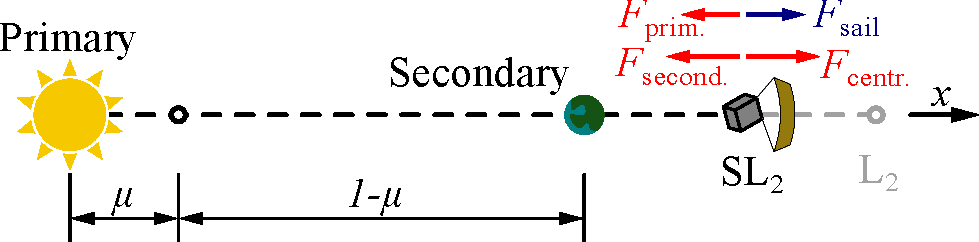
\includegraphics[width=\textwidth]{diagram.pdf}
        \caption{Schematic of all acceleration vectors acting on the spacecraft in the solar sail augmented CR3BP.}
        \label{fig:diagram}
    \end{figure}

    \item[\textbf{2.2}] To verify the required lightness numbers calculations the colinear \acrfull{aep} specified in \cite{heiligers2014} is calculated using this work's implementation and compared to the value reported in the reference, 
    To verify the required lightness numbers calculations the colinear AEP specified in \cite{heiligers2014} is calculated using this work's implementation and compared to the value reported in the reference, 
    the considered case being the Sun--Earth system with a AEP located at $x_{\text{AEP}} = 0.983867$ LU.
    The resulting lightness number is $\beta = 0.0363$, which matches the value reported in \cite{heiligers2014}, confirming the correctness of the implementation. \textit{(64 words)}

    \item[\textbf{2.3}] The required area of the solar sail is derived from the definition of the lightness number:
    \begin{equation}
        \beta \frac{\mu_\odot}{r^2} = 2 P \frac{A}{m} \rightarrow A = \frac{\beta \mu_\odot m}{2 P r^2}
    \end{equation}
    where $m$ is the mass of the spacecraft, $\mu_\odot$ is the gravitational parameter of the Sun ($G M_\odot$), $r$ is the distance from the Sun, and $P$ is the solar radiation pressure at the location of the sail, which can be calculated from the solar constant, $S_{\odot}$ \cite{kopp2011}, and the speed of light, $c$, as follows:
    \begin{equation}
        P = \frac{S_{\odot}}{c} \left( \frac{\text{AU}}{r} \right)^2
    \end{equation}
    The resulting sizes required to achieve the specified shifts in the Lagrange points are shown in Table \ref{tab:sail_area}.\par
    \vspace{1em}
    \begin{table}[htbp]
        \centering
        \caption{Required solar sail side-length to achieve the required shift in the Lagrange points.}
        \label{tab:sail_area}
        \begin{tabular}{lccc}
            \toprule
            \textbf{Lagrange point} & Required solar sail side-length [m] \\
            \midrule
            Sun--Earth L$_2$ & $17.6459$\\
            Sun--Mars L$_2$  & $18.1809$\\
            \bottomrule
        \end{tabular}
    \end{table}
    These sizes are at the upper limit of currently feasible solar sails. The maximum sail size of DCB-based designs in CubeSat form factor is 16.5 m, with larger 
    platforms expected to be capable of deploying sails of up to 22.8 m (\textit{27U HIPERSail}) \cite{wilkie2021ACS3}.

    \item[\textbf{2.4}] To analyse the sensitivity of the required lightness number to the shift in the Lagrange point, a range of 21 shifts from $0.0005$ LU to $0.001$ LU is considered, and the corresponding lightness numbers are computed using the formula from Task 2.1a. The results are shown in Figure \ref{fig:beta_sensitivity}. \par 
    \begin{figure}[htbp]
        \centering
        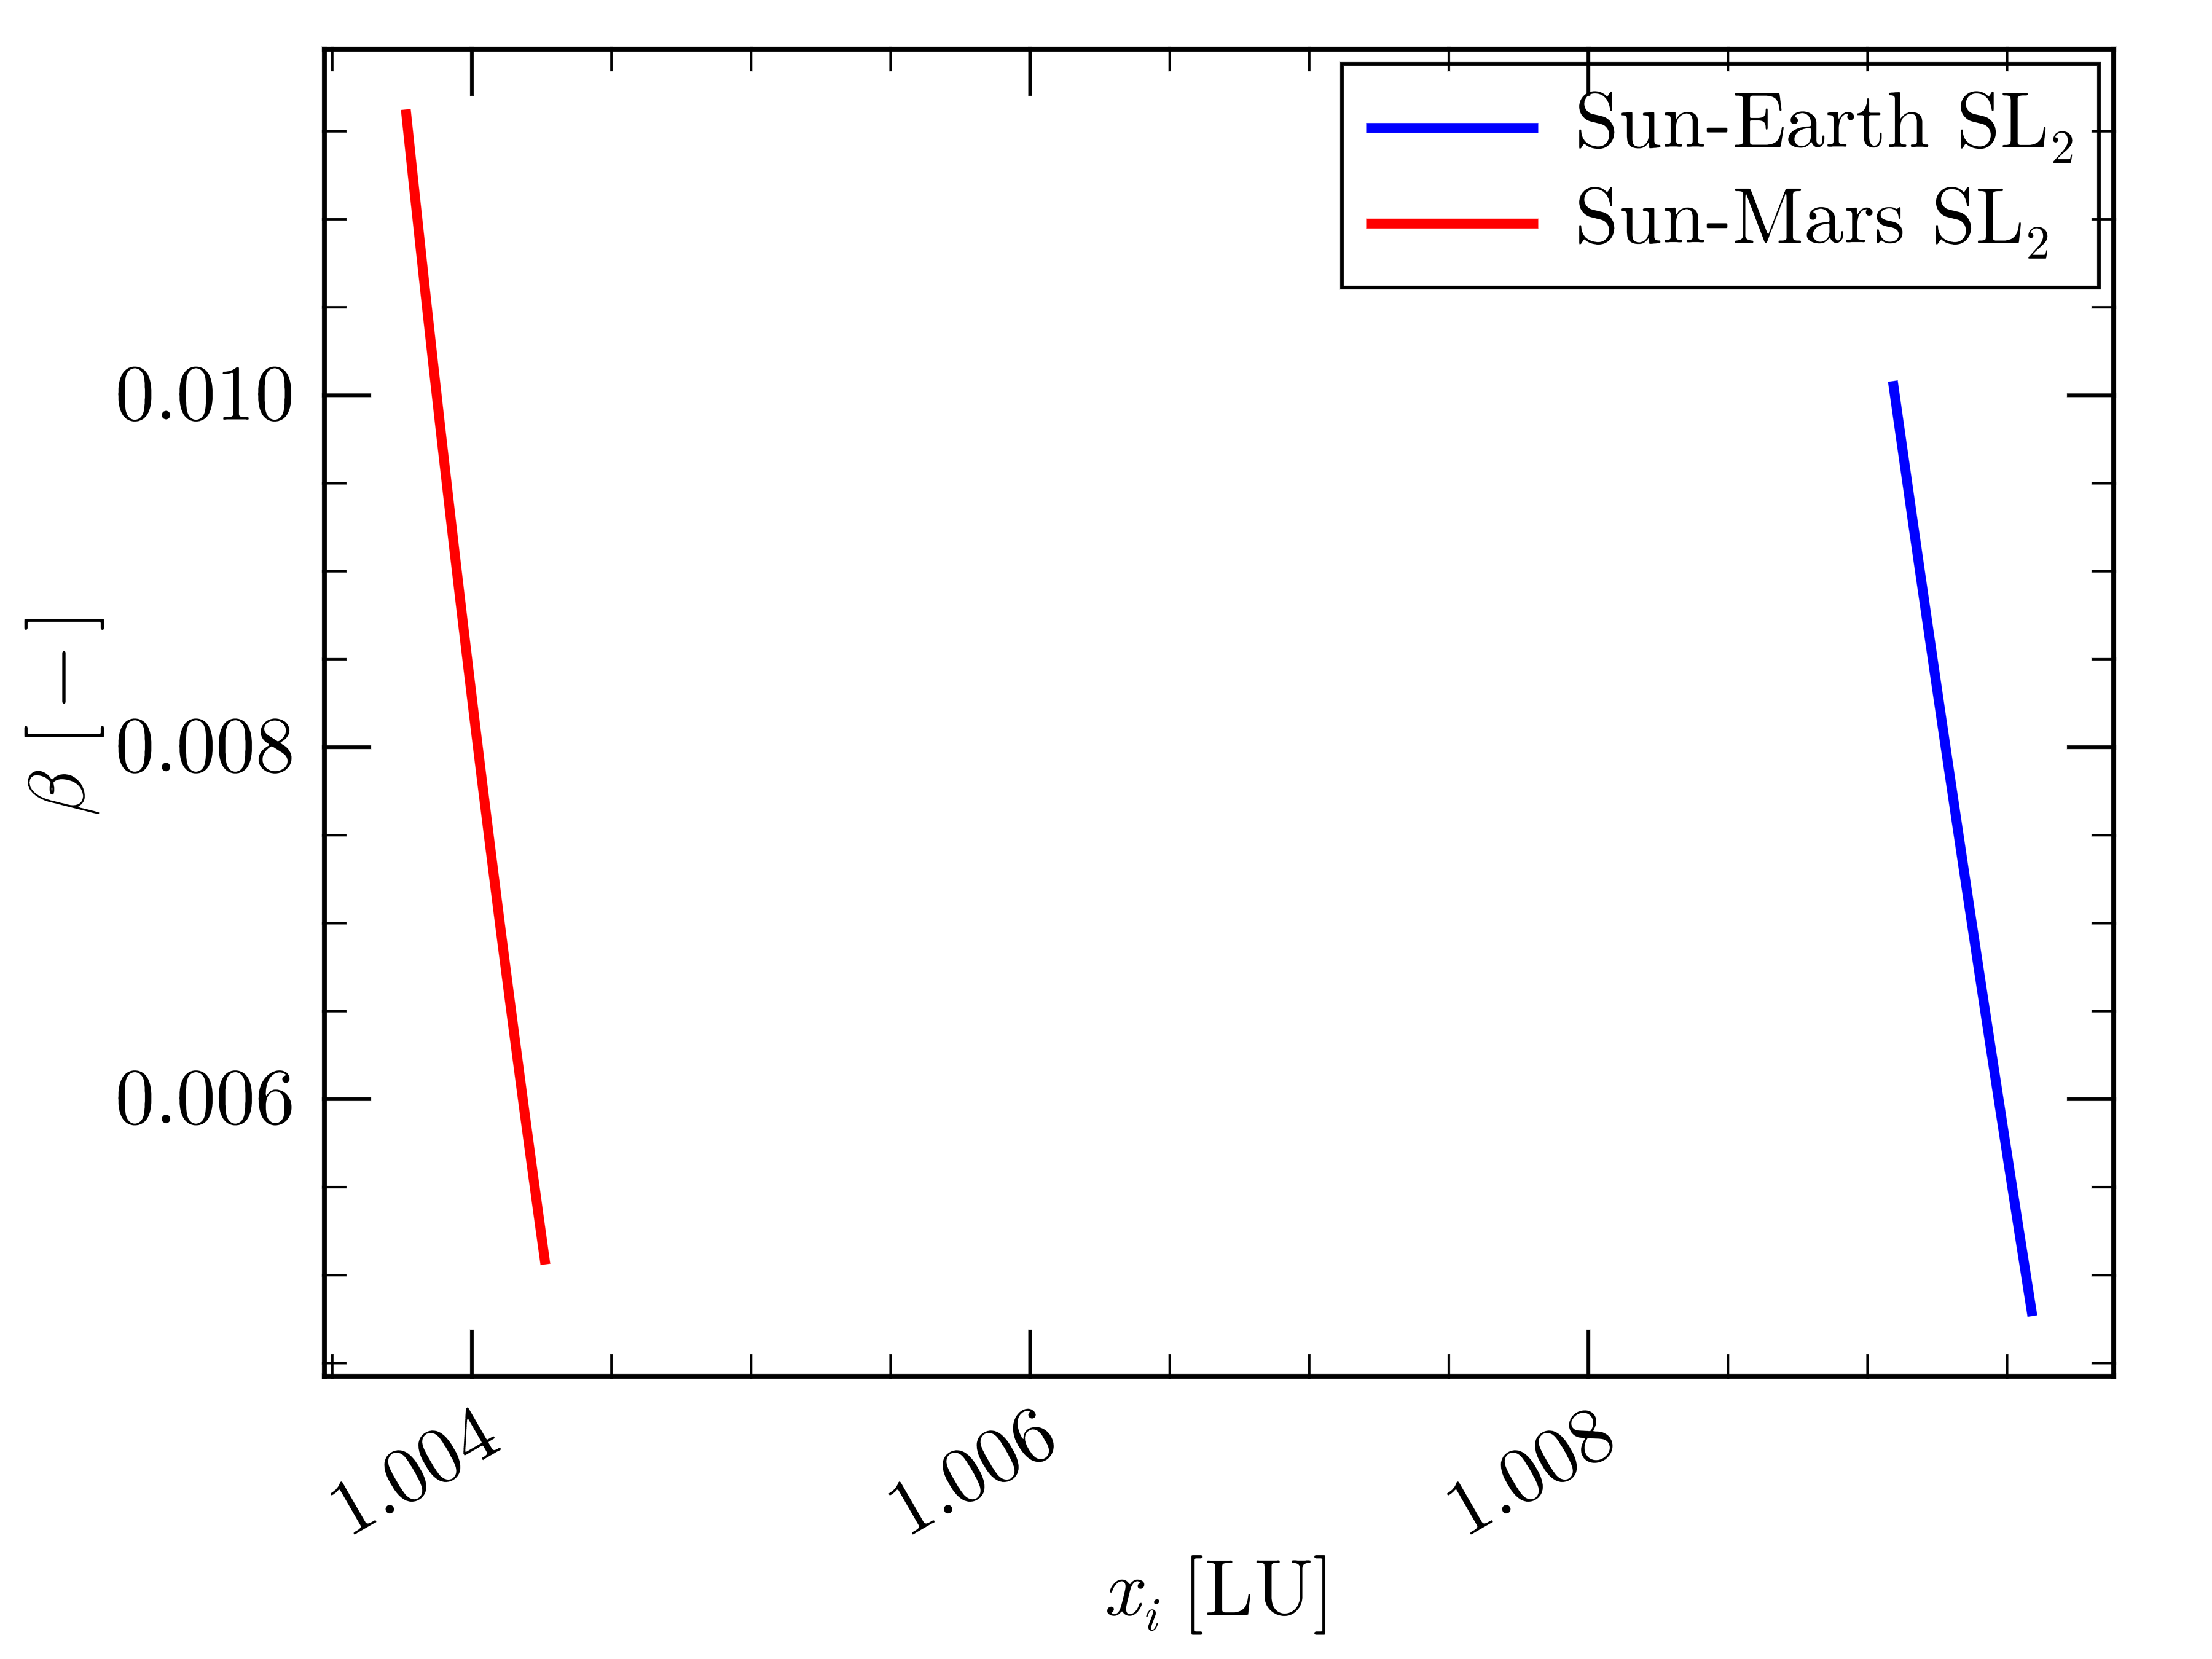
\includegraphics[width=0.75\textwidth]{wp2_beta_sensitivity.png}
        \caption{Sensitivity of the required lightness number, $\beta$, to the shift in the Lagrange point, $\Delta x$, for the Sun--Earth and Sun--Mars systems.}
        \label{fig:beta_sensitivity}
    \end{figure}
    As the equilibrium position moves closer to the planet, the gravitational attraction from both bodies strengthens while the centrifugal acceleration weakens. 
    To counterbalance these effects, the sail acceleration must increase, requiring a larger lightness number. The required $\beta$ is observed to follow a 
    near-linear increase with decreasing distance from the Sun for both systems. \textit{(54 words)}
\end{enumerate}

\newpage
\phantomsection
\section*{WP3 Stability of the (artificial) Lagrange points}
\addcontentsline{toc}{section}{WP3 Stability of the (artificial) Lagrange points}
\label{sec:wp3}

\begin{enumerate}
    \item[\textbf{3.1a}] See Table \ref{tab:eigenvalues}. 

    % \begin{equation}
    %     (\mathbf{a_s})_{ij} = \frac{\partial a_{s,i}}{\partial j} = \bm{\zeta} \mathbf{\hat{n}}^T
    % \end{equation}
    % Where:
    % \begin{equation}
    %     \bm{\zeta} = \frac{4 \beta (1-\mu) (\mathbf{\hat{n}} \cdot \mathbf{\hat{r}_1})}{r_1^3}\left[\frac{\mathbf{\hat{n}}}{2} - (\mathbf{\hat{n}} \cdot \mathbf{\hat{r}_1})\mathbf{\hat{r}_1}\right]
    % \end{equation}
    \vspace{1em}
    \begin{table}[htbp]
        \centering
        \caption{Eigenvalues of the classical and artificial Lagrange points.}        
        \label{tab:eigenvalues}
        \begin{tabular}{lcccc}
            \toprule
            \textbf{Lagrange point} & $\lambda_1$ & $\lambda_2$ & $\lambda_3$ & $\lambda_4$ \\
            \midrule
            Sun--Earth Classical  & $-2.484281$ & $-2.056992i$ & $+2.056992i$ & $+2.484281$ \\
            Sun--Earth Artificial & $-2.673872$ & $-2.174388i$ & $+2.174388i$ & $+2.673872$ \\
            Sun--Mars Classical   & $-2.496888$ & $-2.064657i$ & $+2.064657i$ & $+2.496888$ \\
            Sun--Mars Artificial  & $-2.931888$ & $-2.335453i$ & $+2.335453i$ & $+2.931888$ \\
            \bottomrule
        \end{tabular}
    \end{table}


    \item[\textbf{3.1b}] From the linearization of the problem around the equilibrium points it can be observed that all cases have a positive real eigenvalue, 
    indicating that the nonlinear system is unstable around the equilibrium point \cite{verhulst1996nonlinear}. All eigenvalues take similar values across the 
    4 cases, with slightly higher magnitudes in the Sun--Mars system, indicating faster local dynamics. The introduction of the solar sail also increases the 
    magnitude of all eigenvalues slightly, but not enough to have a qualitative effect on the stability of the system. \textit{(82 words)}

    \item[\textbf{3.2}] For verification purposes the eigenvalue calculation tool results are compared against values preseneted in \cite{szebehely1967theory} for a 
    value of $\mu = 3\times 10^{-6}$. The resulting eigenvalues are shown in Table \ref{tab:eigenvalues_szebehely}.

    \vspace{1em}
    \begin{table}[htbp]
        \centering
        \caption{Verification of the eigenvalue calculation tool for $\mu = 3\times 10^{-6}$.}   
        \label{tab:eigenvalues_szebehely}
        \begin{tabular}{lcccc}
            \toprule
            \textbf{Source} & $\lambda_1$ & $\lambda_2$ & $\lambda_3$ & $\lambda_4$ \\
            \midrule
            This work & $-2.4844225586$ & $-2.0570784929i$ & $+2.0570784929i$ & $+2.4844225586$ \\
            \textcite{szebehely1967theory} & $-2.4844225586$ & $-2.0570784929i$ & $+2.0570784929i$ & $-2.4844225586$ \\
            \bottomrule
        \end{tabular}
    \end{table}

\end{enumerate}

\newpage
\phantomsection
\section*{WP4 Invariant manifolds and application to Mars exploration mission}
\addcontentsline{toc}{section}{WP4 Invariant manifolds and application to Mars exploration mission}
\label{sec:wp4}

\begin{enumerate}
    \item[\textbf{4.1}] See Figure \ref{fig:classical-manifolds}
    \begin{figure}[htbp]
        \centering
        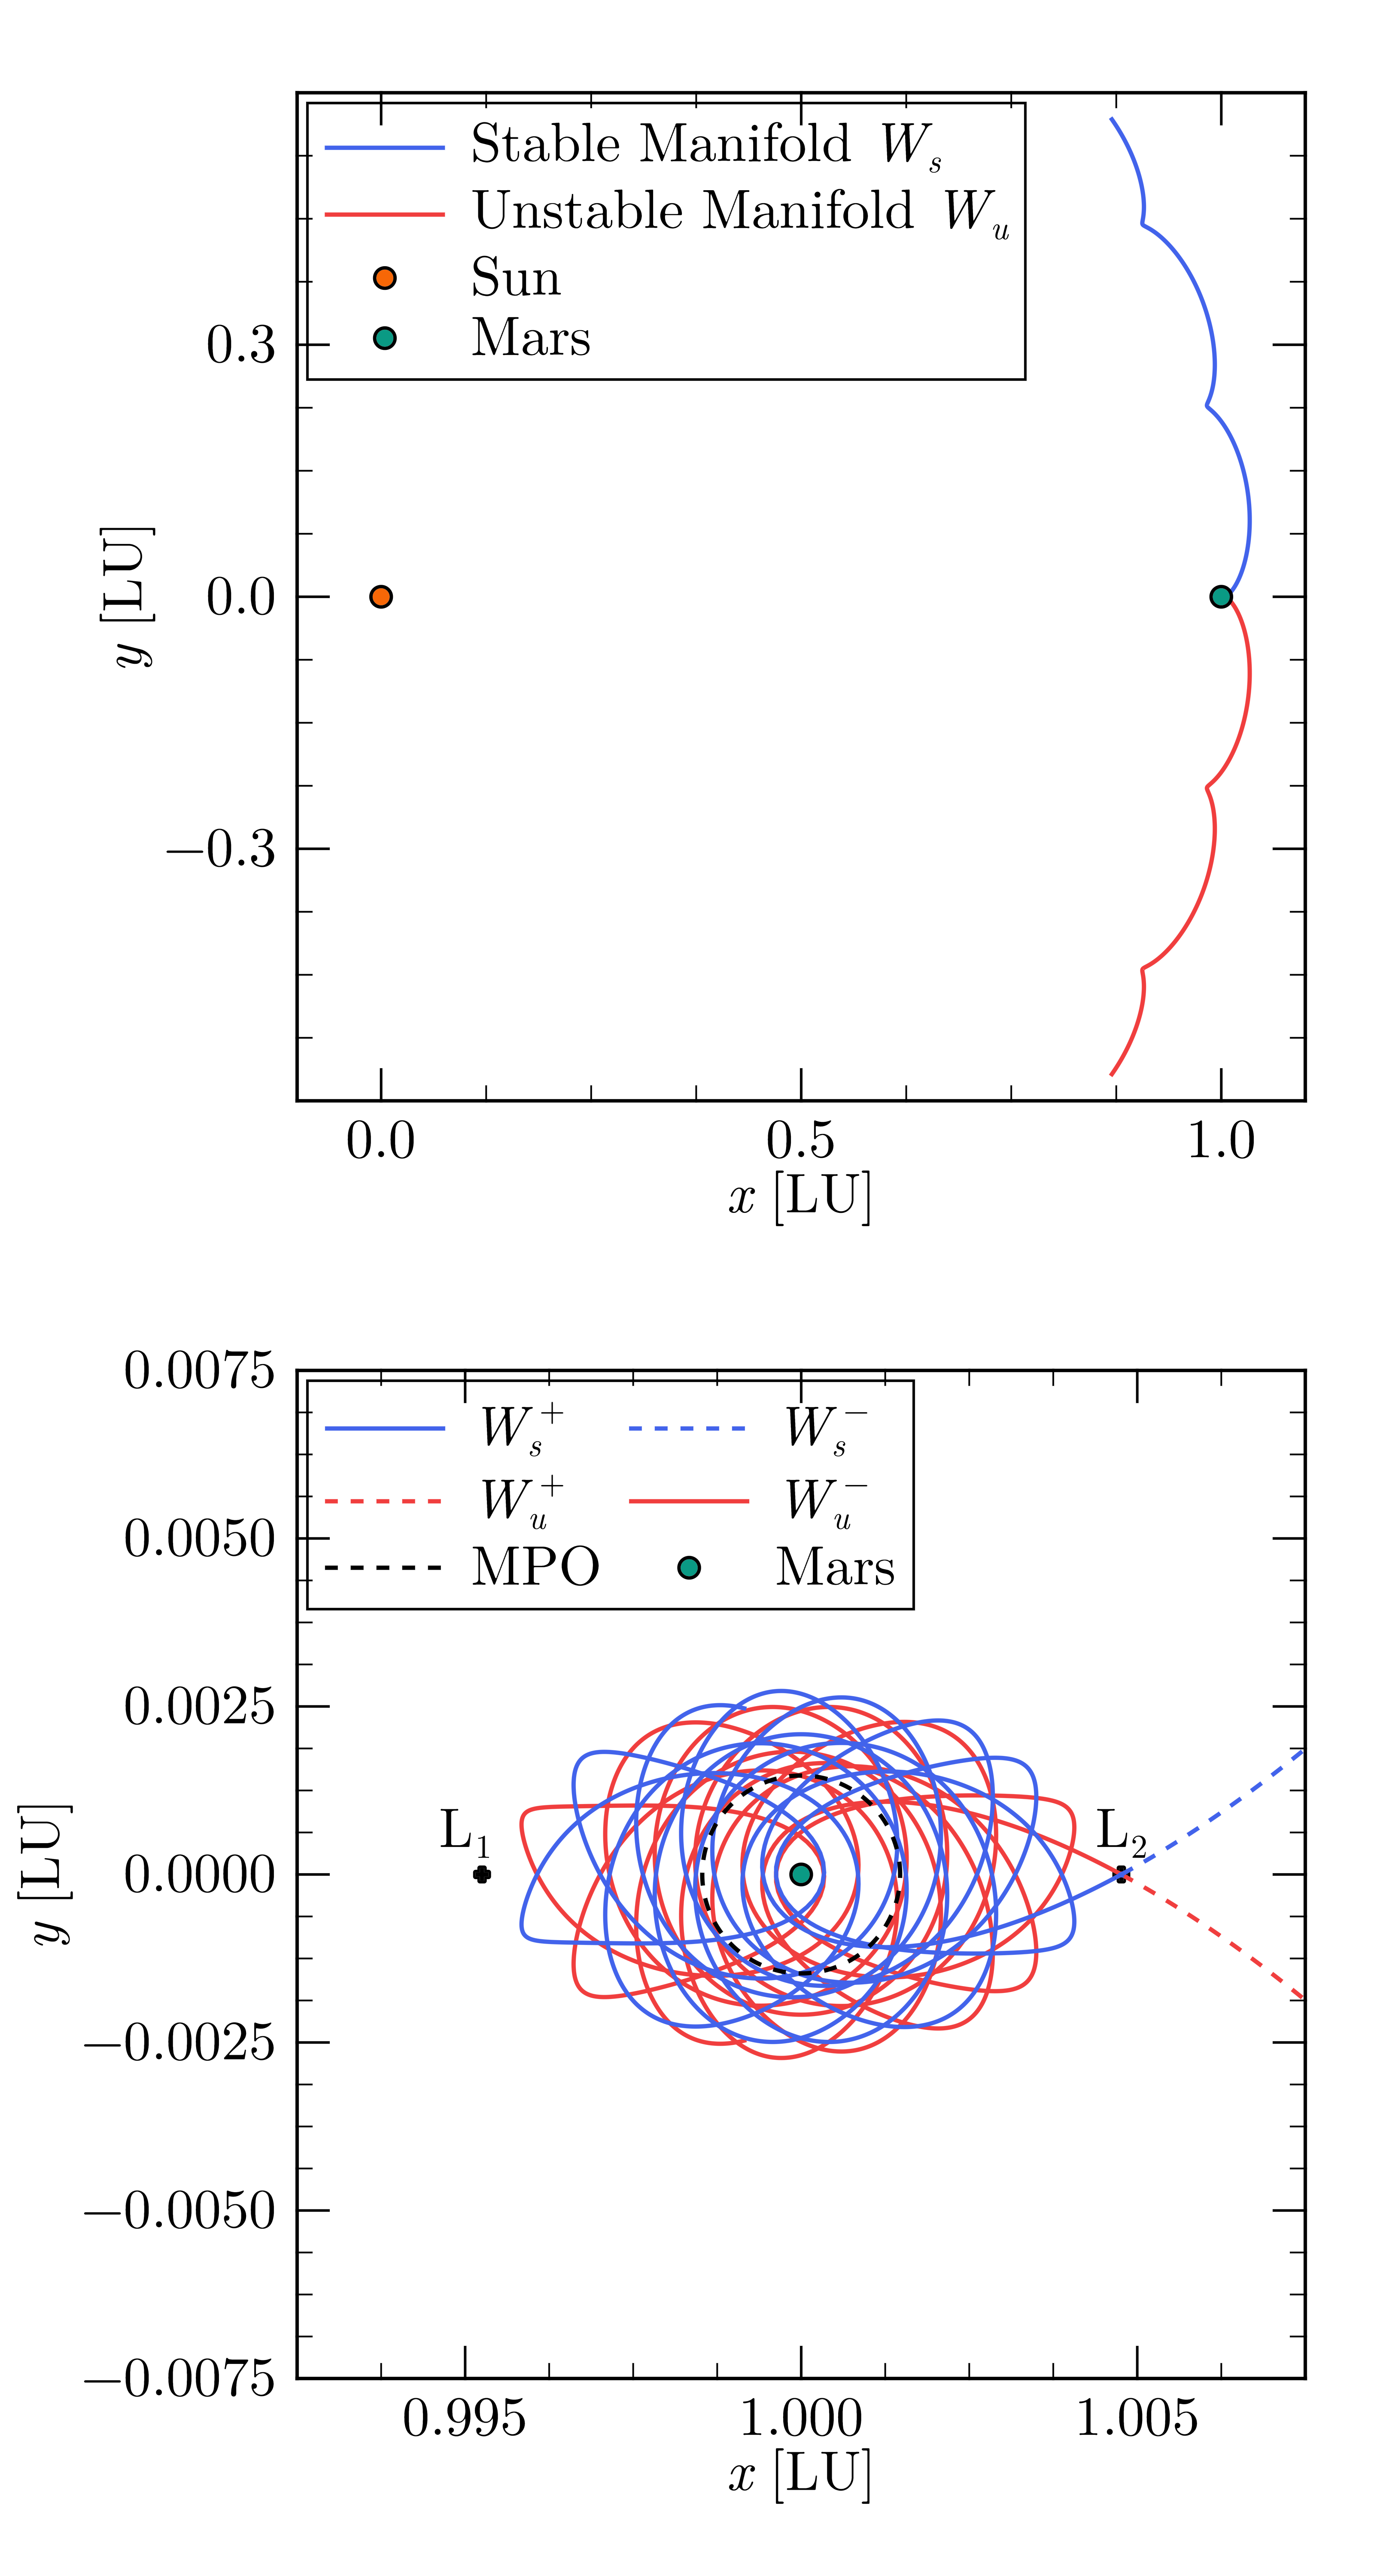
\includegraphics[width=0.75\textwidth]{wp41_manifolds.png}
        \caption{Stable($W^s$) and unstable($W^u$) invariant manifolds of the classical L$_2$ point in the Sun--Mars system.}
        \label{fig:classical-manifolds}
    \end{figure}

    \item[\textbf{4.2a}] The unstable manifold departing L$_2$ intersects the \acrfull{mpo}, enabling a propulsion-free transfer. However, 
    the manifolds do not intersect Earth's orbit, as it lies on a different energy level, meaning propulsion is required for the Earth to Sun--Mars L$_2$ leg. \textit{(40 words)}

    \item[\textbf{4.2b}] See Table \ref{tab:deltaV-classical} and Figure \ref{fig:leg2-classical}.
    \vspace{1em}
    \begin{table}[htbp]
        \centering
        \caption{$\Delta V$s required to establish a natural transfer between Earth and Mars.}   
        \label{tab:deltaV-classical}
        \begin{tabular}{ccc}
            \toprule
            $\Delta V_\text{E}$ [m/s] & $\Delta V_\text{M}$ [m/s] & $\Delta V_\text{TOT}$ [m/s] \\
            \midrule
            -- & 294.0023 & 294.0023 \\
            \bottomrule
        \end{tabular}
    \end{table}
    \begin{figure}[htbp]
        \centering
        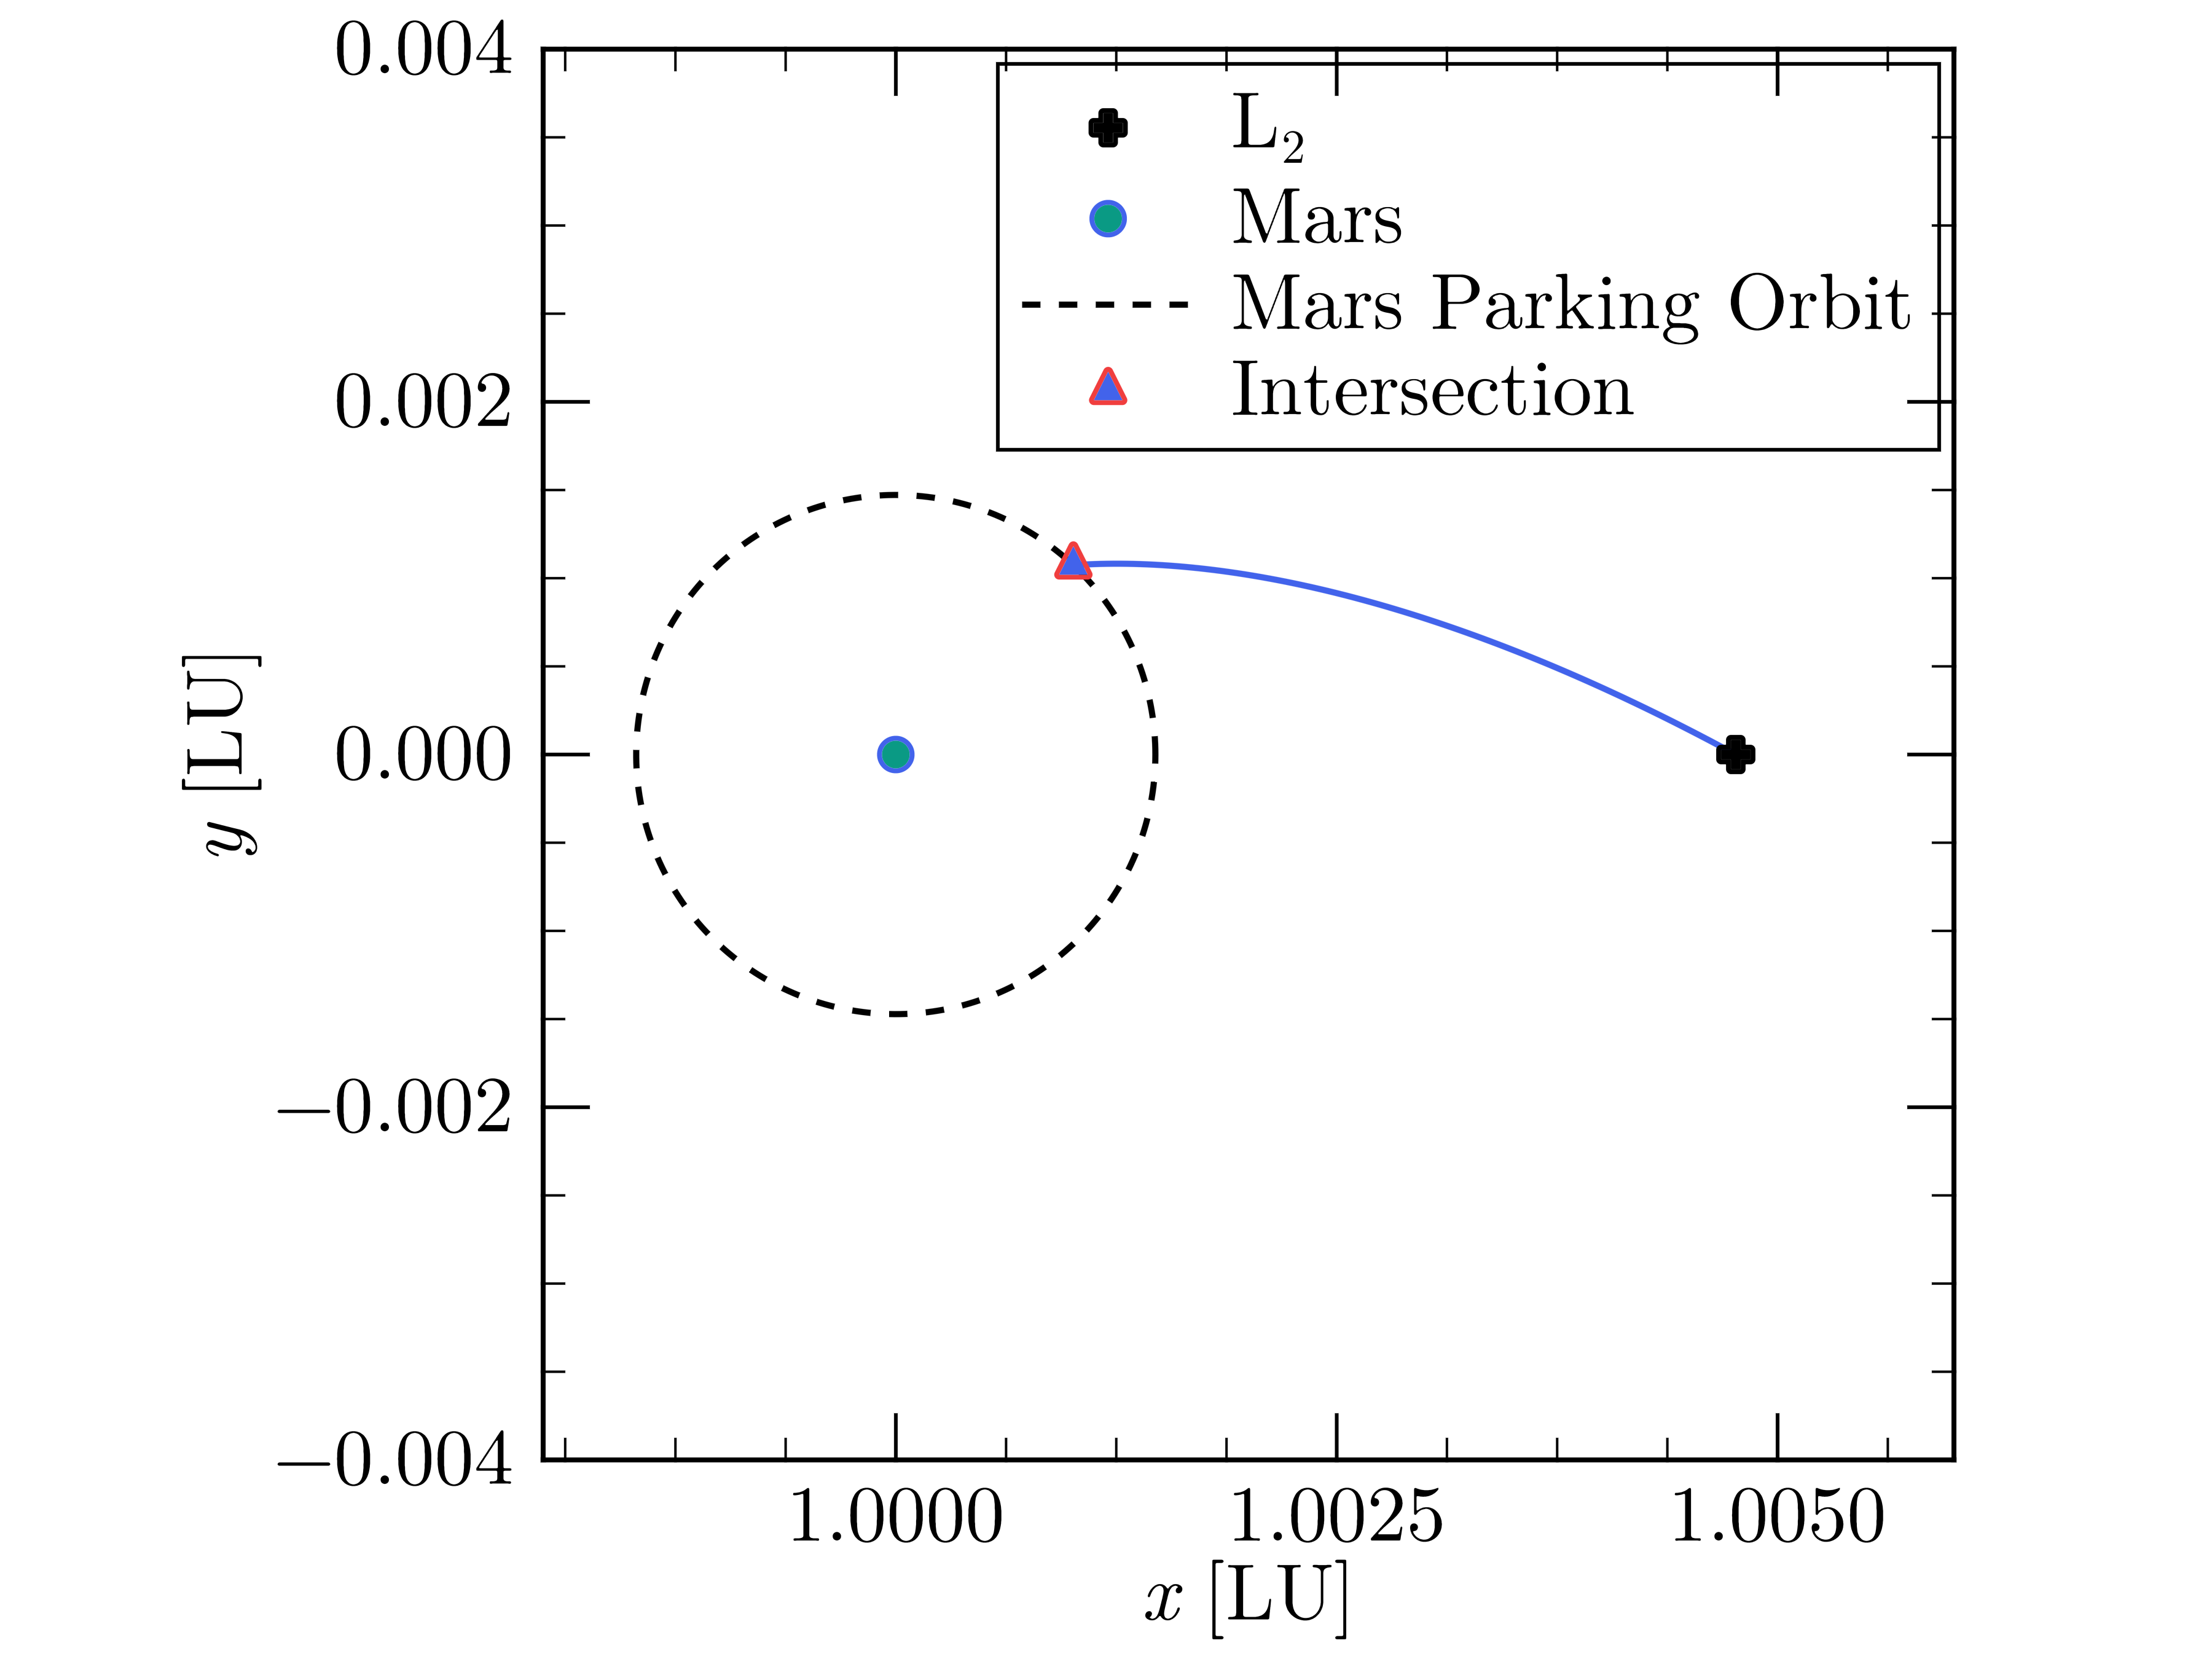
\includegraphics[width=0.75\textwidth]{wp42_mars_transfer.png}
        \caption{Close up of the natural transfer from L$_2$ to the MPO.}
        \label{fig:leg2-classical}
    \end{figure}

    \item[\textbf{4.3}] See Table \ref{tab:solar sail-transfer} and Figures \ref{fig:deltaV-ss} and \ref{fig:optimal-transfer}.
    \begin{figure}[htbp]
        \centering
        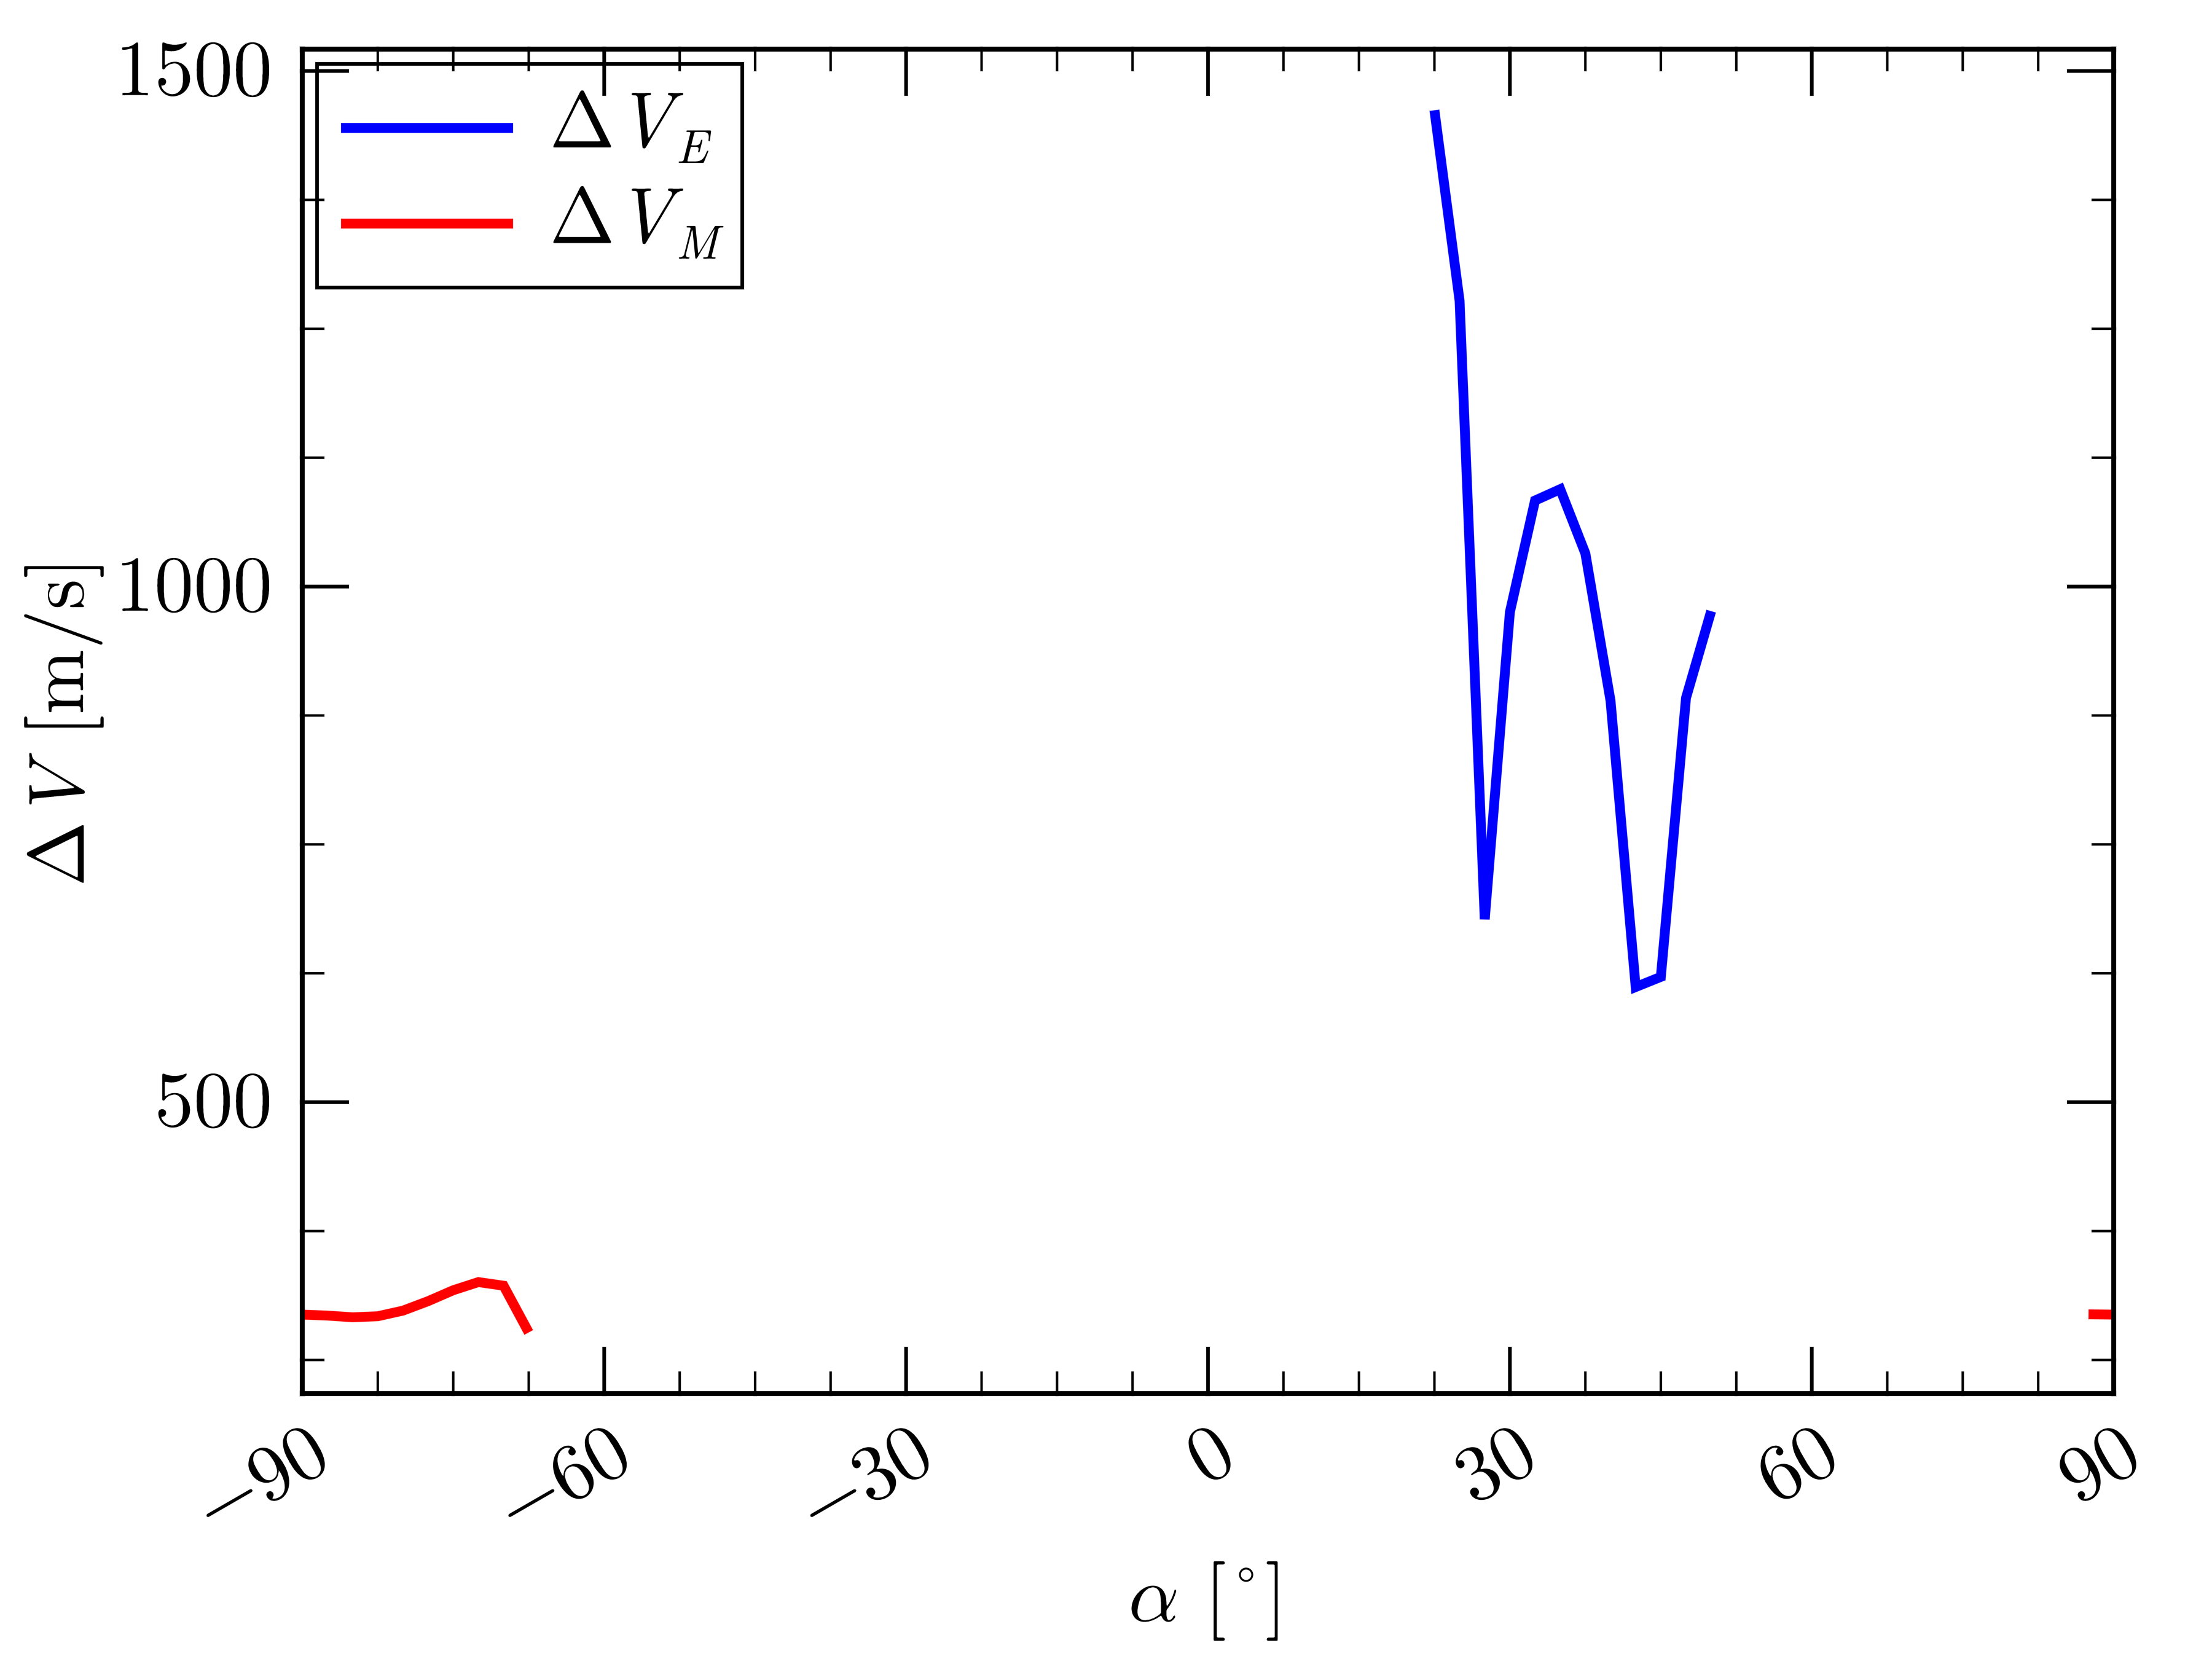
\includegraphics[width=0.75\textwidth]{wp43_deltav_vs_alpha.png}
        \caption{$\Delta V$s of the solar sail transfer as a function of the cone angle.}
        \label{fig:deltaV-ss}
    \end{figure}
    \vspace{1em}
    \begin{table}[htbp]
        \centering
        \caption{Details of the solar sail Earth--Mars transfer with the smallest total $\Delta V$, $\Delta V_\text{TOT}$.}
        \label{tab:solar sail-transfer}
        \begin{tabular}{ccccccc}
            \toprule
            \makecell{Leg 1 \\ optimal \\ cone \\ angle [$^\circ$]} &
            \makecell{Leg 2 \\ optimal \\ cone \\ angle [$^\circ$]} &
            $\Delta V_\text{E}$ [m/s] &
            $\Delta V_\text{M}$ [m/s] &
            $\Delta V_\text{TOT}$ [m/s] &
            \makecell{Time of \\ Flight Leg 1 \\ \ [Earth years]} &
            \makecell{Time of \\ Flight Leg 2 \\ \ [Earth years]} \\
            \midrule
            42.5 & -67.5 & 611.6762 & 276.6996 & 888.3757 & 4.0092 & 0.5521 \\
            \bottomrule
        \end{tabular}
    \end{table}
    \begin{figure}[htbp]
        \centering
        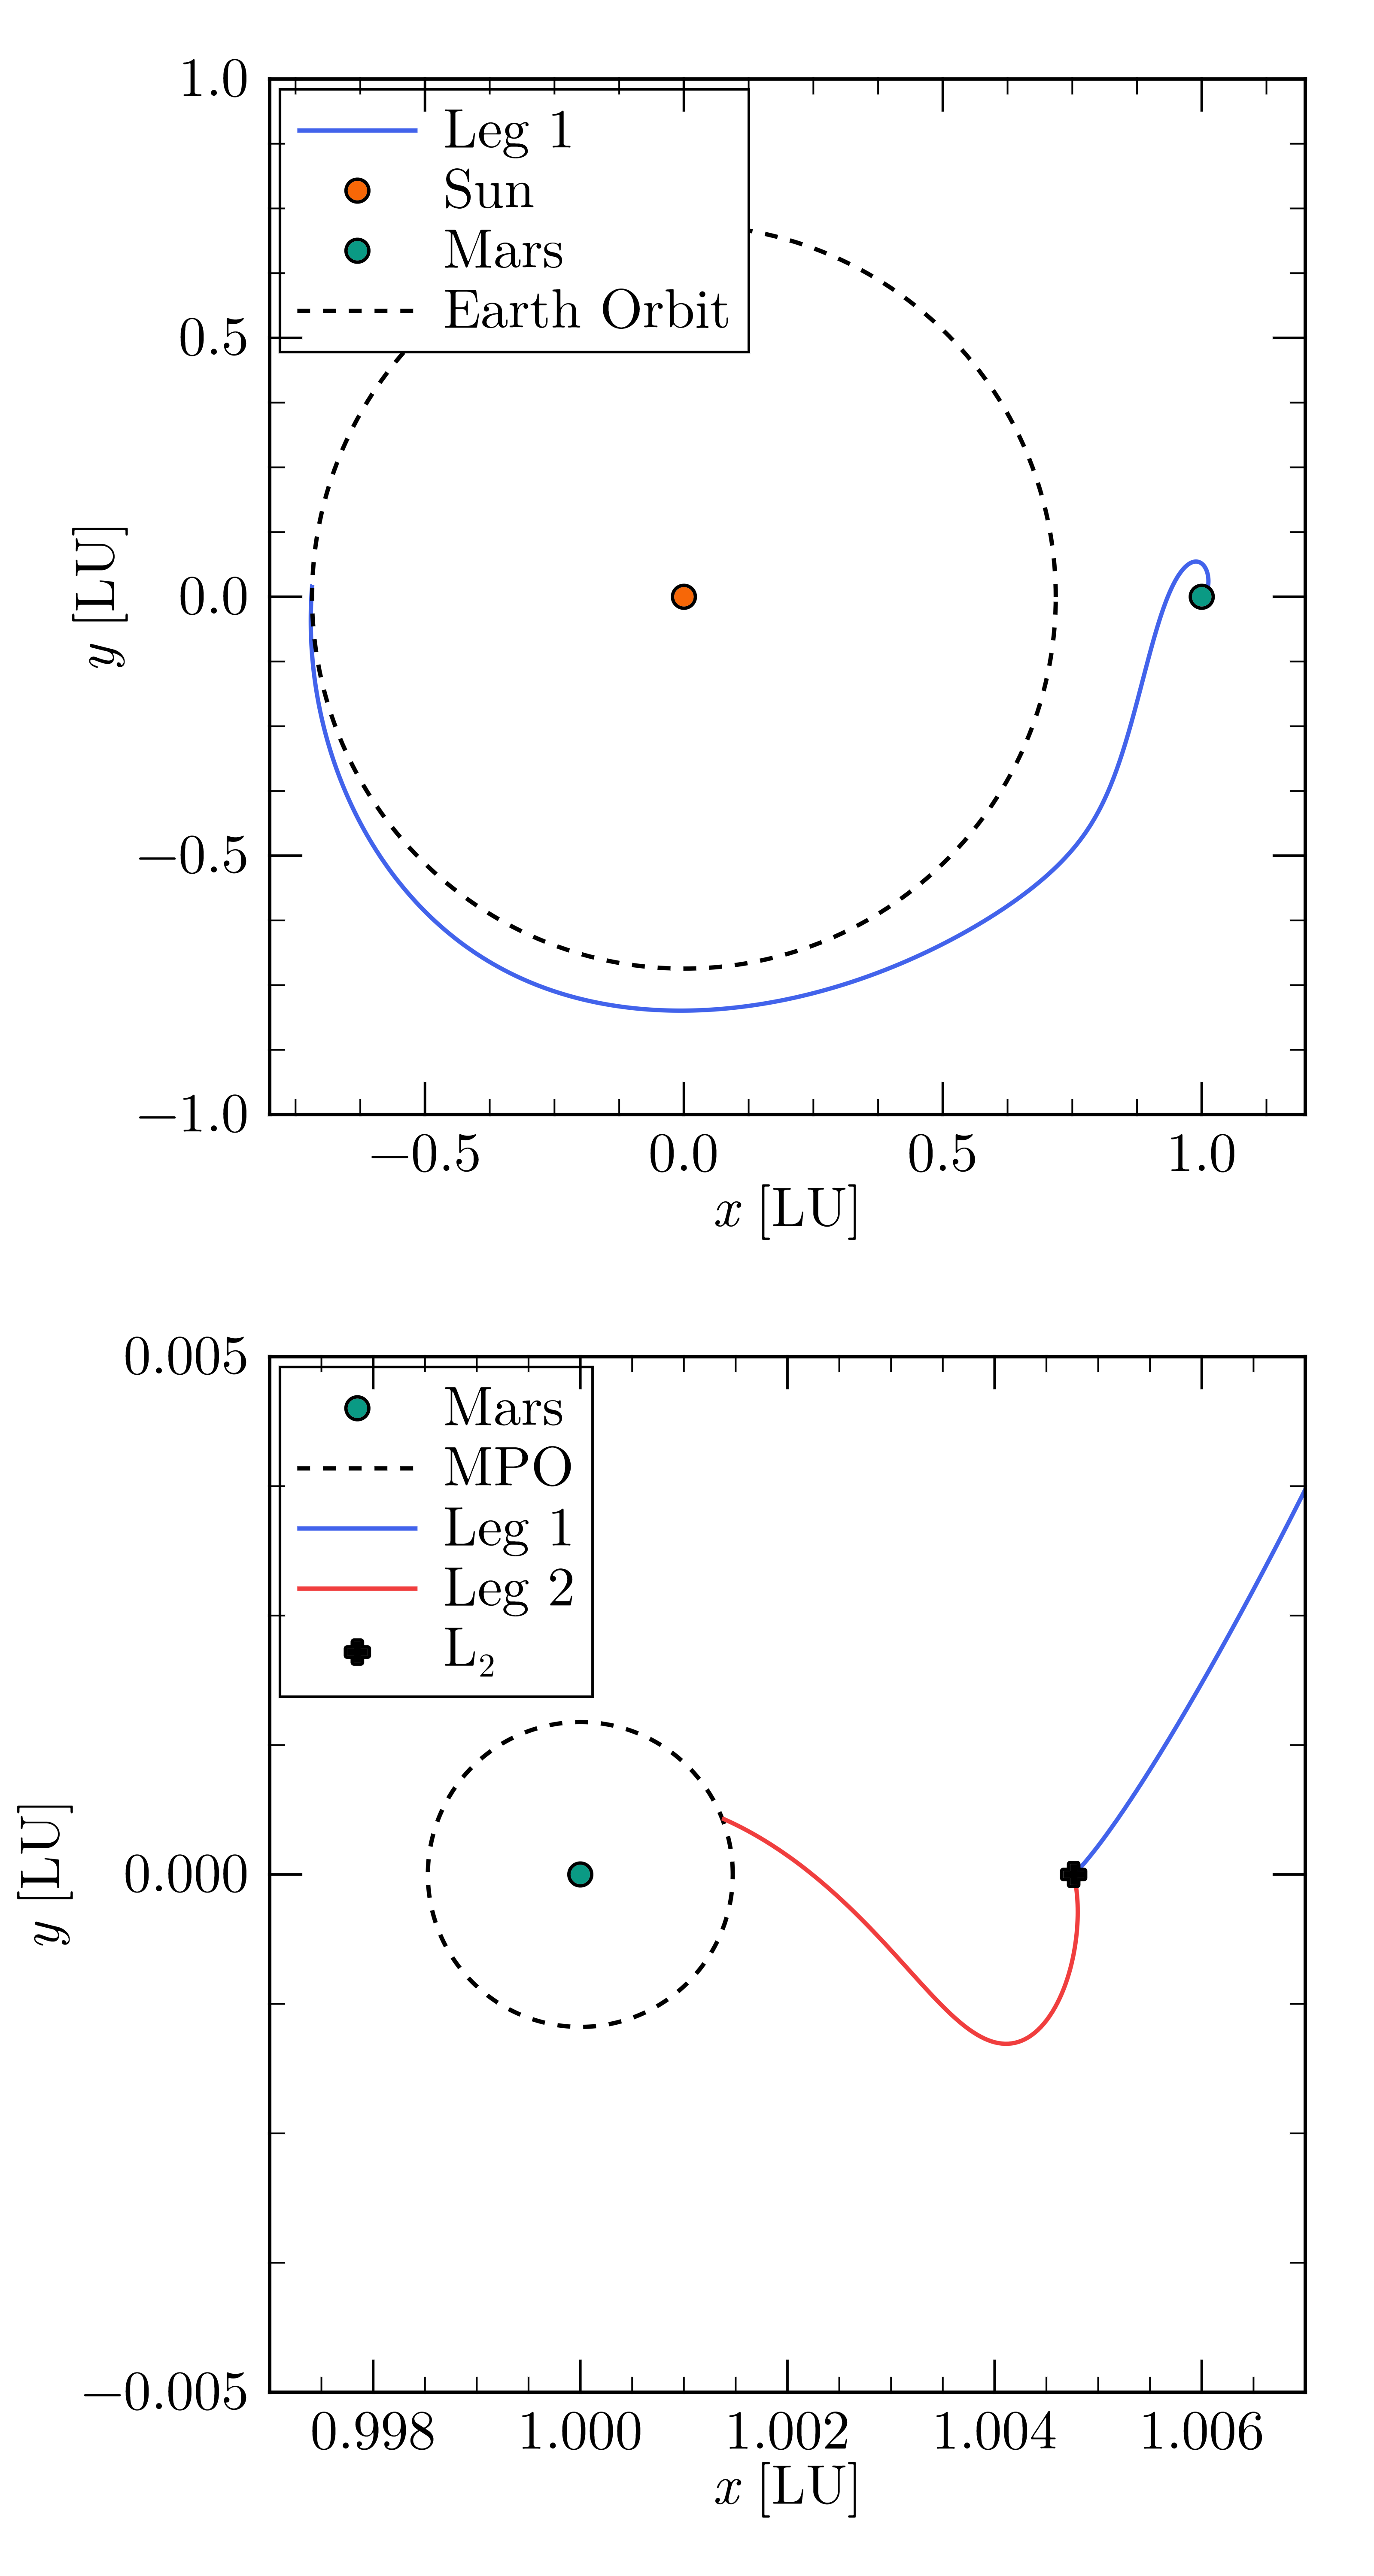
\includegraphics[width=0.75\textwidth]{wp43_optimal_transfers.png}
        \caption{Optimal transfer trajectory from Earth to the MPO via the Sun--Mars L$_2$ point using a solar sail.}
        \label{fig:optimal-transfer}
    \end{figure}

    \item[\textbf{4.4}] 

    \item[\textbf{4.5}] The earliest possible departure date for the optimal transfer is determined by the synodic mean anomaly of the Earth and Mars as follows:
    \begin{equation*}
        t_{\text{dep}} = \frac{\mod(\theta_\text{dep} - \theta_0, 2\pi)}{n_E - n_M} + t_0
    \end{equation*}
    The earliest departure date is found to be on the \textbf{25th of May, 2030}.
    
    \item[\textbf{4.6}] The results demonstrate that solar sail missions from Earth to Mars with minimized $\Delta V$ are feasible. However, several limitations
     constrain practical applicability. The assumed 100 kg spacecraft is already at the boundary of current solar sail technology, and the true useful payload 
     is further reduced by the mass of sail support systems, attitude control hardware, propulsion systems for the required $\Delta V$ maneuvers, and Mars
      descent mechanisms, none of which have been accounted for in this study. This makes the small payload the primary limiting factor for the exploitation of 
      this technology in the near term.
    \par
    A viable niche may nonetheless emerge in the long term. In the short term, Mars settlement will rely primarily on in-situ resource utilization 
    \cite{zamani2024feasibility}, but once sustained settlements with predictable long-term supply demands are established, low-cost propellant-efficient 
    delivery architectures of this kind could play a meaningful supporting role. \textit{(144 words)}

\end{enumerate}

% \begin{figure}[htbp]
%     \centering
%     % \includegraphics[width=0.75\textwidth]{figures/example.pdf}
%     \rule{0.75\textwidth}{4cm}  % placeholder; replace with \includegraphics
%     \caption{Caption describing the figure. Include units and clarify all
%              curves or data series shown.}
%     \label{fig:example}
% \end{figure}
% 
% \begin{table}[htbp]
%     \centering
%     \caption{Summary of simulation parameters.}
%     \label{tab:example}
%     \begin{tabular}{llS[table-format=4.3]}
%         \toprule
%         Parameter       & Symbol    & {Value} \\
%         \midrule
%         Semi-major axis & $a$       & 6778.137 \\
%         Eccentricity    & $e$       & 0.000 \\
%         Inclination     & $i$       & 28.500 \\
%         \bottomrule
%     \end{tabular}
% \end{table}

% REFERENCES
\clearpage
\newpage
\printbibliography[heading=bibintoc, title={References}]

%  APPENDICES
% \newpage
% \appendix
% 
% \section{Appendix Title}
% \label{app:A}
% 
% Include supplementary derivations, raw data tables, or code listings here.
% Appendices are labelled A, B, C, etc., automatically.
% 
% \lipsum[7]

\end{document}